\documentclass[11pt,compress,t,notes=noshow, aspectratio=169, xcolor=table]{beamer}

\usepackage{../../style/lmu-lecture}
% Defines macros and environments
% This file is included in slides and exercises

% Rarely used fontstyle for R packages, used only in 
% - forests/slides-forests-benchmark.tex
% - exercises/single-exercises/methods_l_1.Rnw
% - slides/cart/attic/slides_extra_trees.Rnw
\newcommand{\pkg}[1]{{\fontseries{b}\selectfont #1}}

% Spacing helpers, used often (mostly in exercises for \dlz)
\newcommand{\lz}{\vspace{0.5cm}} % vertical space (used often in slides)
\newcommand{\dlz}{\vspace{1cm}}  % double vertical space (used often in exercises, never in slides)
\newcommand{\oneliner}[1] % Oneliner for important statements, used e.g. in iml, algods
{\begin{block}{}\begin{center}\begin{Large}#1\end{Large}\end{center}\end{block}}

% Don't know if this is used or needed, remove?
% textcolor that works in mathmode
% https://tex.stackexchange.com/a/261480
% Used e.g. in forests/slides-forests-bagging.tex
% [...] \textcolor{blue}{\tfrac{1}{M}\sum^M_{m} [...]
% \makeatletter
% \renewcommand*{\@textcolor}[3]{%
%   \protect\leavevmode
%   \begingroup
%     \color#1{#2}#3%
%   \endgroup
% }
% \makeatother


\title{Interpretable Machine Learning}
% \author{LMU}
%\institute{\href{https://compstat-lmu.github.io/lecture_iml/}{compstat-lmu.github.io/lecture\_iml}}
\date{}

%\bibliography{feature-importance}

%\usepackage{Sweave}
\begin{document}
	\newcommand{\titlefigure}{figure_man/feature-importance.png}
    \newcommand{\learninggoals}{
    	\item Definition of LOCO
    	\item Interpretation of LOCO}
	% Set style/preamble. Rnw as parent.
	
	% Load all R packages and set up knitr
	
	% This file loads R packages, configures knitr options and sets preamble.Rnw as 
	% parent file
	% IF YOU MODIFY THIS, PLZ ALSO MODIFY setup.Rmd ACCORDINGLY...
	
	% Defines macros and environments

	\lecturechapter{Leave One Covariate Out (LOCO)}
	\lecture{Interpretable Machine Learning}
	
	% ------------------------------------------------------------------------------

%TODO: Remove gray figure background (e.g. theme_bw())

% \begin{frame}{Reminder: Feature Importance Scheme}
% In general, feature importance methods share two components
% \lz
% \begin{enumerate}
%   \item \textbf{Perturbation/Removal:} Generate predictions for which the feature of interest has been perturbed/removed.
%   \item \textbf{Performance Comparision:} Compare performance under perturbation/removal with the original model performance.
% \end{enumerate}
% \lz
% Depending on the type of perturbation/removal feature importance methods provide insight into different aspects of model and data.\\
% \lz
% \textbf{LOCO idea:} Simply remove the feature from the dataset and refit the model on the reduced dataset. The performance loss compared to the full model is interpreted as feature importance.\\

% \end{frame}

\begin{frame}{LOCO \citebutton{Lei et al. (2018)}{https://arxiv.org/abs/1604.04173} \citebutton{Tibshirani (2018)}{http://www.stat.cmu.edu/~ryantibs/talks/loco-2018.pdf}}
% citation of the original LOCO paper
%
\textbf{LOCO idea:} Remove the feature from data, refit model on reduced data, and measure the loss in performance compared to model fitted on complete data. %Remove the feature from the dataset and refit the model on the reduced dataset. The performance loss compared to the full model is interpreted as feature importance.

\pause\medskip

%\textbf{Definition:} Given train and test data $\Dtrain, \Dtest \subseteq \D$, for learner $\ind$ and model $\fh = \ind(\Dtrain)$. Then LOCO for a feature $j \in \pset$ can be computed as follows:
\textbf{Definition:} Given train and test data $\Dtrain, \Dtest \subseteq \D$, a learner $\ind$, and model $\fh := \ind(\Dtrain)$, the LOCO importance for feature $j \in \pset$ is computed by:

\medskip

  \begin{enumerate}
    \item Learn model on ${\Dtrain}_{,-j}$ where feature $x_j$ was removed, i.e. $\fh_{-j} = \ind({\Dtrain}_{,-j})$\pause
    \item Compute the difference in local $L_1$ loss for each element in $\Dtest$, i.e. $\Delta_j^{(i)} = \left  |y^{(i)} - \fh_{-j}(x_{-j}^{(i)}) \right | - \left |y^{(i)} - \fh(x^{(i)}) \right | $ with $i \in \Dtest$\pause
    \item Compute importance score by $\text{LOCO}_j = \text{med} \left ( \Delta_j  \right )$
  \end{enumerate}

\medskip\pause

The method can be generalized to other loss functions and aggregations. If we use mean instead of median we can rewrite LOCO as
%
$$ \text{LOCO}_j = \riske(\fh_{-j}) - \riske(\fh).$$
%\footnote[frame]{\fullcite{lei_distribution-free_2018}\\ \fullcite{tibshirani_loco_2018}}
\end{frame}

\begin{frame}{Bike Sharing Example}
%
\begin{figure}
  \centering
  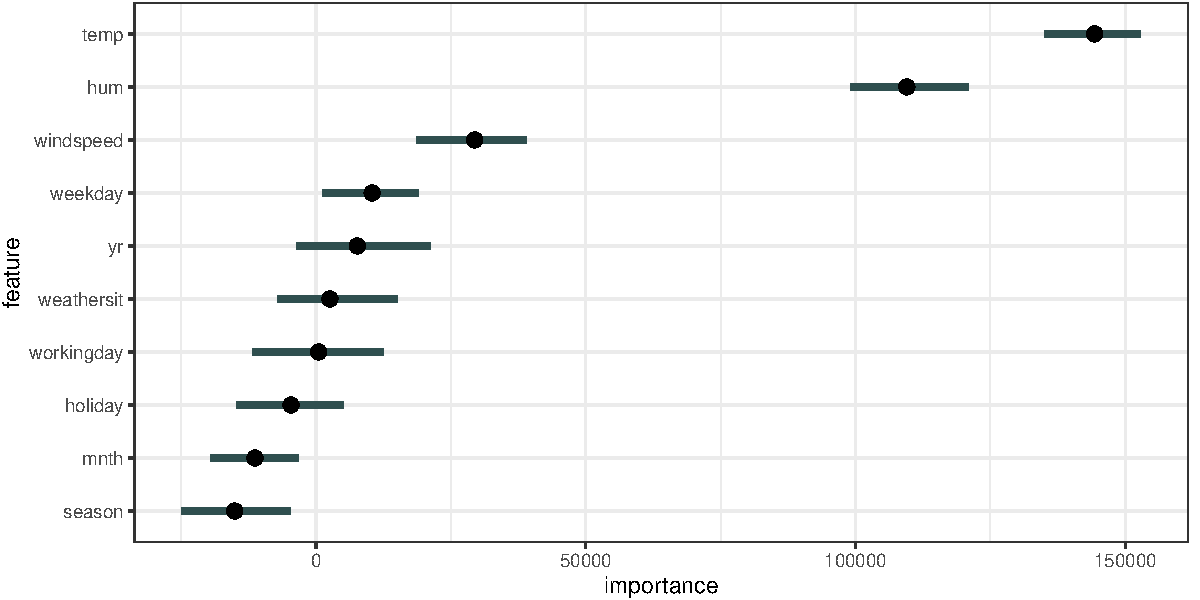
\includegraphics[width=\textwidth]{figure_man/bike_sharing_loco.pdf}
%\caption{A random forest with default hyperparameters was fit on $70\%$ of the bike sharing data (training set) to optimize MSE. Then LOCO was computed for all features on the test data. The temperature is the most important feature. Without access to \texttt{temp}, the MSE increases by approx. $140,000$.}
\end{figure}
%
 %\textbf{Interpretation:} $\text{LOCO}_j$ quantifies how important variable $x_j$ is to the generalization performance of the learner on $\Dtrain$.\\
%
\begin{itemize}
  \item Trained random forest (default hyperparameters) on 70\% of bike sharing data
  \item Performance measure: mean squared error (MSE)
  \item Computed LOCO on test set for all features, measuring increase in MSE
  \item \texttt{temp} was most important: removing it increased MSE by approx. $140.000$
\end{itemize}

\end{frame}

\begin{frame}{Interpretation of LOCO}

\textbf{Interpretation:} LOCO estimates the generalization error of the learner on a reduced dataset $\D_{-j}$.\\
\lz
Can we get insight into whether the ...
\begin{enumerate}
    \item feature $x_j$ is causal for the prediction $\yh$?
    \begin{itemize}
      \item In general, no also because we refit the model (counterexample next slide)
    \end{itemize}
    \item feature $x_j$ contains prediction-relevant information?
    \begin{itemize}
      \item In general, no (counterexample on the next slide)
    \end{itemize}
    \item model requires access to $x_j$ to achieve its prediction performance?
    \begin{itemize}
      \item Approximately, it provides insight into whether the \textit{learner} requires access to $x_j$
    \end{itemize}
\end{enumerate}
\end{frame}

\begin{frame}{Interpretation of LOCO}



% x1 = rnorm(n, mean=0, sd = 5)
% x2 = rnorm(n, mean=0, sd = 0.1) + x1
% x3 = rnorm(n, mean=0, sd = 5)
% y = rnorm(n, mean = 0, sd = 2) + x3 + x2

\textbf{Example:} Sample $1000$ observations with
\begin{itemize}
    \item $x_1, x_3 \sim N(0, 5)$,  $x_2 = x_1 + \epsilon_2$ with $\epsilon_2 \sim N(0, 0.1)$
    \item $y = x_2 + x_3 + \epsilon$ with $\epsilon \sim N(0, 2)$
    \item Trained LM: $\fh(x) = -0.02 - 1.02 x_1 + 2.05 x_2 + 0.98 x_3$
\end{itemize}

%Sample $1000$ observations with $x_1, x_3 \sim N(0, 5), x_2 = x_1 + \epsilon_2$ with $\epsilon_2 \sim N(0, 0.1)$ and $y = x_2 + x_3 + \epsilon$ with $\epsilon \sim N(0, 2)$.

\pause

\begin{columns}[c, totalwidth=\textwidth]
\begin{column}{0.42\textwidth}
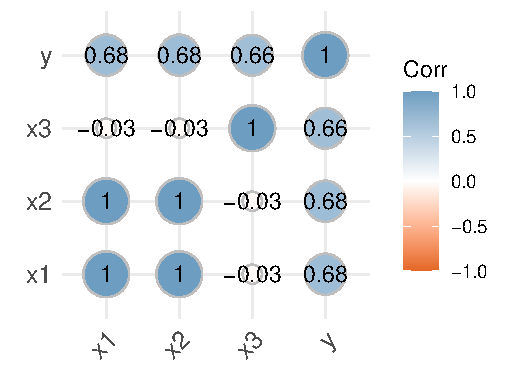
\includegraphics[width=\linewidth]{figure_man/simulation_loco_corr.pdf}\\
\centerline{Correlation matrix}

\end{column}
\begin{column}{0.58\textwidth}
\centering
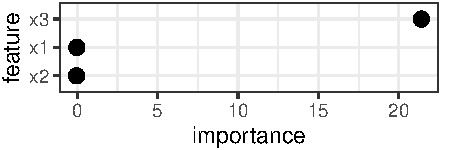
\includegraphics[width=0.9\linewidth]{figure_man/simulation_loco}\\
LOCO importance from LM trained on 70\% of data, evaluated on remaining 30\%
%LOCO importance of LM fitted on 70\% of the data computed on 30\% remaining observations
%\begin{figure}
%\centering
%\hfill
 % \begin{tikzpicture}[thick, scale=1.1, every node/.style={scale=0.6, line width=0.3mm, black, fill=white}]
%		\node[draw, circle, font=\large] (x1) at  (-.5, 2) {$X_1$};
%		\node[draw, circle, font=\large] (x2) at  (-.5,1) {$X_2$};
%		\node[draw, circle, font=\large] (x3) at  (.5,1) {$X_3$};
%		\node[draw, circle, font=\large] (y) at  (0,0) {$Y$};
%		\draw[->, black] (x1) -- (x2);
%		\draw[->, black] (x3) -- (y);
%		\draw[->, black] (x2) -- (y);
%	\end{tikzpicture} 
%\hfill
% 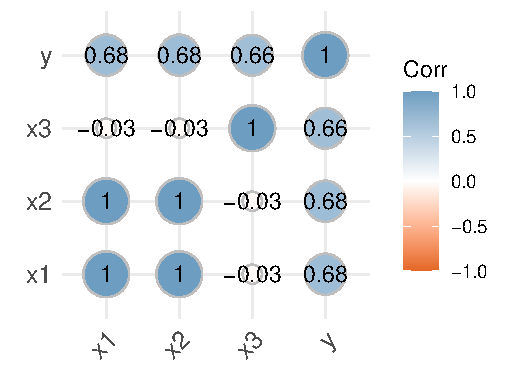
\includegraphics[width=\linewidth]{figure_man/simulation_loco_corr.pdf} 
% \hfill
% 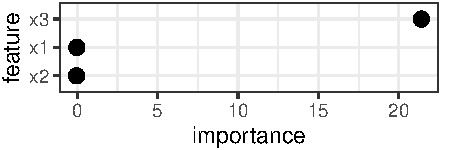
\includegraphics[width=\linewidth]{figure_man/simulation_loco}
%\hfill
%\end{figure}

%Linear Gaussian data generating process with correlation matrix as depicted left.
%A linear model was fit with $\fh(x) = -0.09 - 0.86 x_1 + 1.86 x_2 + 0.96 x_3$.\\

\end{column}
\end{columns}

\lz\pause

$\Rightarrow$ We cannot infer (1) from LOCO (e.g. $\text{LOCO}_2 \approx 0$ but coefficient of $x_2$ is $2.05$)\\\pause
$\Rightarrow$ We also can't infer (2), e.g., $Cor(x_2, y) = 0.68$ but $\text{LOCO}_2 \approx 0$\\\pause
$\Rightarrow$ We can get insight into (3): $x_2$ and $x_1$ highly correlated with $\text{LOCO}_1 = \text{LOCO}_2  \approx 0$ \\
\phantom{$\Rightarrow$} $\leadsto$ $x_2$ and $x_1$ take each others place if one of them is left out (not the case for $x_3$)
%As $x_2$ and $x_1$ are highly correlated, they can take each others place, which is not the case for $x_3$.
\end{frame}

%TODO: Why only?
\begin{frame}{Pros and Cons}
  Pros:
  \begin{itemize}
    \item Requires (only?) one refitting step per feature for evaluation
    \item Easy to implement
    \item Testing framework available in \citebutton{Lei et al. (2018)}{https://arxiv.org/abs/1604.04173}
  \end{itemize}
%
  Cons:
  \begin{itemize}
    \item Provides insight into a learner on specific data, not a specific model\\
    $+$ for algorithm-level insight\\
    $-$ for model-specific insights
    %Does not provide insight into a specific model, but rather a learner on a specific dataset
    \item Model training is a random process and LOCO estimates can be noisy\\
    $\leadsto$ Limits inference about on model and data, or multiple refittings necessary?
    \item Requires re-fitting the learner for each feature\\
    $\leadsto$ Computationally intensive compared to PFI
  \end{itemize}
\end{frame}

%\begin{frame}{Bibliography}
%  \printbibliography
%\end{frame}

\endlecture
\end{document}
